\documentclass[11pt,a4paper]{article}

% --- Packages ---
\usepackage[utf8]{inputenc}
\usepackage[T1]{fontenc}
\usepackage{lmodern}
\usepackage[margin=2.2cm]{geometry}
\usepackage{xcolor}
\usepackage{parskip}
\usepackage{enumitem}
\usepackage{booktabs}
\usepackage{array}
\usepackage{tabularx}
\usepackage{tikz}
\usetikzlibrary{arrows.meta, positioning, shapes.geometric, calc, shadows, fadings}
\usepackage[most]{tcolorbox}
\tcbuselibrary{skins, breakable}
\usepackage[hidelinks,colorlinks=true,urlcolor=blue!60!black,linkcolor=black]{hyperref}
\usepackage{titling}
\usepackage{titlesec}
\usepackage{qrcode}

% --- Colors ---
\definecolor{accent}{HTML}{2A6F97}
\definecolor{accent2}{HTML}{61A5C2}
\definecolor{warnbg}{HTML}{FFF4E6}
\definecolor{warnframe}{HTML}{D97706}
\definecolor{tipbg}{HTML}{ECFDF5}
\definecolor{tipframe}{HTML}{059669}
\definecolor{promptbg}{HTML}{F4F4F8}
\definecolor{promptframe}{HTML}{6B7280}
\definecolor{toolbg}{HTML}{EAF3F9}
% Phase palette for the pipeline diagram
\definecolor{phaseFind}{HTML}{2A6F97}        % deep blue
\definecolor{phaseUnderstand}{HTML}{8E44AD}  % muted purple
\definecolor{phaseCreate}{HTML}{059669}      % green
\definecolor{trail}{HTML}{B8C5D6}            % soft track
\definecolor{ink}{HTML}{2D3748}              % off-black for text

% --- Boxes ---
\newtcolorbox{watchout}[1][]{
  enhanced, breakable,
  colback=warnbg, colframe=warnframe,
  fonttitle=\bfseries, title=Watch out,
  left=8pt, right=8pt, top=4pt, bottom=4pt,
  boxrule=0.5pt, arc=2pt, #1
}
\newtcolorbox{tipbox}[1][]{
  enhanced, breakable,
  colback=tipbg, colframe=tipframe,
  fonttitle=\bfseries, title=Tip,
  left=8pt, right=8pt, top=4pt, bottom=4pt,
  boxrule=0.5pt, arc=2pt, #1
}
\newtcolorbox{promptbox}[1][]{
  enhanced,
  colback=promptbg, colframe=promptframe,
  fonttitle=\bfseries, title=Copy-paste prompt,
  left=8pt, right=8pt, top=4pt, bottom=4pt,
  boxrule=0.5pt, arc=2pt, fontupper=\small\ttfamily, #1
}
\newtcolorbox{toolheader}[1][]{
  enhanced,
  colback=toolbg, colframe=accent,
  left=10pt, right=10pt, top=6pt, bottom=6pt,
  boxrule=0.6pt, arc=3pt, #1
}

% --- Titles ---
\titleformat{\section}
  {\Large\bfseries\color{accent}}{\thesection}{0.6em}{}
\titleformat{\subsection}
  {\large\bfseries\color{accent!85!black}}{\thesubsection}{0.6em}{}

% --- Document metadata ---
\title{\textbf{From Topic to Talk in One Pipeline}\\[2pt]
\large A 45-minute practical with five AI research tools}
\author{LOURIM, AI for Research Seminar Series, Part 1\\\small Practical session, Corentin Vande Kerckhove}
\date{8 May 2026}

\begin{document}
\maketitle

\begin{tcolorbox}[colback=accent!8, colframe=accent!50, left=10pt, right=10pt, top=6pt, bottom=6pt, boxrule=0.4pt, arc=3pt]
\textbf{What you will do today.} You received a research topic on a slip of paper, randomly assigned by a peer. By the end of this session you will have \emph{started} a pipeline that ends, at home, with two deliverables:
\begin{itemize}[leftmargin=1.2em, itemsep=1pt, topsep=2pt]
  \item a short \textbf{document} that gives an overview of recent progress in the field and lays out a few promising research questions attached to it;
  \item a \textbf{slide deck} built from that document, which you can reuse to pitch the questions and find potential collaborators.
\end{itemize}
You will email both to a researcher working in the field, asking which of those questions might be worth pursuing. The five tools below each take care of one step.
\end{tcolorbox}

\vspace{0.6em}
\begin{center}
\begin{tabular}{@{}c@{\hspace{1em}}l@{}}
\qrcode[height=2.2cm]{https://github.com/cvandekerckh/lourim-ai-seminar-series} &
\begin{minipage}[c]{0.55\linewidth}
\small\textbf{Scan to open the source repo.}\\
All slides, this tutorial, and the upcoming seminar materials live at\\
\href{https://github.com/cvandekerckh/lourim-ai-seminar-series}{github.com/cvandekerckh/lourim-ai-seminar-series}.
\end{minipage}
\end{tabular}
\end{center}

\setcounter{tocdepth}{1}
\tableofcontents
\vspace{0.5em}

\clearpage
% =====================================================================
\section{Overview}
\label{sec:overview}

\subsection{From topic to talk: the method}

Before we name any tool, here is the recipe behind doing good research, with or without AI. Five steps, in order:

\vspace{0.6em}
\begin{center}
\resizebox{0.92\linewidth}{!}{%
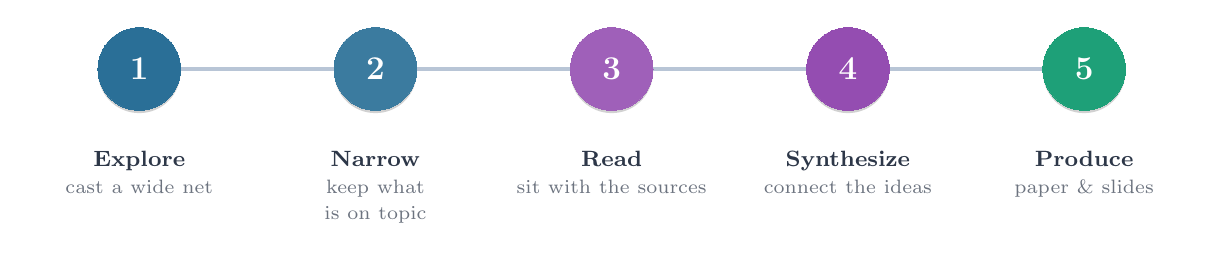
\begin{tikzpicture}[
  every node/.style={font=\footnotesize, color=ink},
  mstep/.style={
    circle, draw=phaseFind, fill=phaseFind, line width=0pt,
    minimum size=1.05cm, text=white, font=\bfseries\large,
    drop shadow={shadow xshift=0pt, shadow yshift=-1pt, opacity=0.18, fill=black}
  },
  mcap/.style={align=center, text width=2.6cm, anchor=north}
]
% trail line
\draw[line width=1.4pt, color=trail] (0,0) -- (12,0);

% steps
\node[mstep] (s1) at (0,0)  {1};
\node[mstep, fill=phaseFind!92, draw=phaseFind!92] (s2) at (3,0)  {2};
\node[mstep, fill=phaseUnderstand!85, draw=phaseUnderstand!85] (s3) at (6,0)  {3};
\node[mstep, fill=phaseUnderstand!95, draw=phaseUnderstand!95] (s4) at (9,0)  {4};
\node[mstep, fill=phaseCreate!90, draw=phaseCreate!90] (s5) at (12,0) {5};

% captions
\node[mcap, yshift=-4mm] at (s1.south) {\textbf{Explore}\\\scriptsize\color{ink!70}cast a wide net};
\node[mcap, yshift=-4mm] at (s2.south) {\textbf{Narrow}\\\scriptsize\color{ink!70}keep what is on topic};
\node[mcap, yshift=-4mm] at (s3.south) {\textbf{Read}\\\scriptsize\color{ink!70}sit with the sources};
\node[mcap, yshift=-4mm] at (s4.south) {\textbf{Synthesize}\\\scriptsize\color{ink!70}connect the ideas};
\node[mcap, yshift=-4mm] at (s5.south) {\textbf{Produce}\\\scriptsize\color{ink!70}paper \& slides};
\end{tikzpicture}%
}%
\end{center}
\vspace{0.6em}

\textbf{Explore.} You start from a topic, not a question. Look broadly at what already exists, even outside your own field, so you do not miss the literature that matters.

\textbf{Narrow.} Filter the long initial list into a small, trustworthy set you can actually engage with. Drop the off-topic and the weak.

\textbf{Read.} Spend real time with each source. Note the question it asks, the method it uses, what it finds, and where it is fragile.

\textbf{Synthesize.} Step out of individual papers and look at the picture they make together: what is the consensus, where do they disagree, what is missing?

\textbf{Produce.} Turn that synthesis into something other people can engage with: a written argument for the open research questions you found, and a presentation that does it justice.

This recipe is the work of any researcher. The five AI tools below are nothing more than \emph{assistants} for each step. They speed up the recipe, they do not replace it.

\subsection{The five tools}

Each tool takes care of one step of the recipe and answers one specific question:

\vspace{0.4em}
\begin{center}
\resizebox{\linewidth}{!}{%
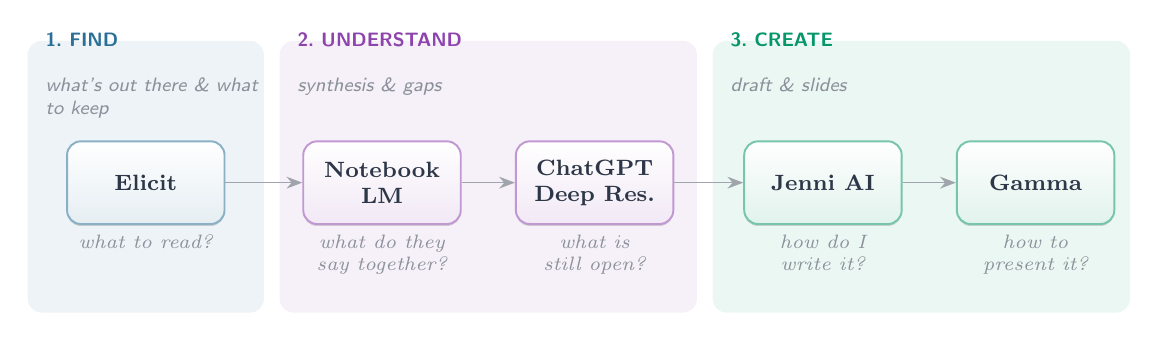
\begin{tikzpicture}[
  every node/.style={font=\footnotesize, color=ink},
  pill/.style={
    rectangle, rounded corners=5pt,
    fill=white, line width=0.7pt,
    minimum width=2.0cm, minimum height=1.05cm,
    align=center, inner sep=3pt,
    drop shadow={shadow xshift=0pt, shadow yshift=-0.7pt, opacity=0.16, fill=black}
  },
  arr/.style={-{Stealth[length=2mm]}, draw=ink!45, line width=0.55pt},
  phaseLabel/.style={
    font=\bfseries\sffamily\scriptsize, anchor=south west, inner sep=2pt
  },
  phaseSub/.style={
    font=\sffamily\scriptsize\itshape, anchor=north west, color=ink!55, inner sep=2pt,
    text width=2.9cm, align=left
  },
  question/.style={
    font=\scriptsize\itshape, anchor=north, color=ink!55,
    align=center, text width=2.2cm
  }
]
% --- Phase background ribbons ---
\fill[phaseFind!8, rounded corners=5pt] (-0.20, -1.65) rectangle (2.80, 1.80);
\fill[phaseUnderstand!8, rounded corners=5pt] (3.00, -1.65) rectangle (8.30, 1.80);
\fill[phaseCreate!8, rounded corners=5pt] (8.50, -1.65) rectangle (13.80, 1.80);

% --- Phase labels (label on top line, italic descriptor on line below) ---
\node[phaseLabel, color=phaseFind]      at (-0.05, 1.65) {1.\ FIND};
\node[phaseSub]                          at (-0.05, 1.40) {what's out there \& what to keep};

\node[phaseLabel, color=phaseUnderstand] at (3.15, 1.65) {2.\ UNDERSTAND};
\node[phaseSub]                          at (3.15, 1.40) {synthesis \& gaps};

\node[phaseLabel, color=phaseCreate]     at (8.65, 1.65) {3.\ CREATE};
\node[phaseSub]                          at (8.65, 1.40) {draft \& slides};

% --- Tool pills ---
\node[pill, draw=phaseFind!55, top color=white, bottom color=phaseFind!12] (el) at (1.30, 0.00) {\textbf{Elicit}};

\node[pill, draw=phaseUnderstand!55, top color=white, bottom color=phaseUnderstand!12] (nb) at (4.30, 0.00) {\textbf{Notebook}\\\textbf{LM}};
\node[pill, draw=phaseUnderstand!55, top color=white, bottom color=phaseUnderstand!12] (cg) at (7.00, 0.00) {\textbf{ChatGPT}\\\textbf{Deep Res.}};

\node[pill, draw=phaseCreate!55, top color=white, bottom color=phaseCreate!12] (jn) at (9.90, 0.00) {\textbf{Jenni AI}};
\node[pill, draw=phaseCreate!55, top color=white, bottom color=phaseCreate!12] (gm) at (12.60, 0.00) {\textbf{Gamma}};

% --- Per-tool questions (below pills) ---
\node[question] at (el.south) {what to read?};
\node[question] at (nb.south) {what do they say together?};
\node[question] at (cg.south) {what is still open?};
\node[question] at (jn.south) {how do I write it?};
\node[question] at (gm.south) {how to present it?};

% --- Flow arrows ---
\draw[arr] (el) -- (nb);
\draw[arr] (nb) -- (cg);
\draw[arr] (cg) -- (jn);
\draw[arr] (jn) -- (gm);

\end{tikzpicture}%
}%
\end{center}
\vspace{0.4em}

\subsection{Time budget}

The 45-minute session is a \textbf{kickoff}, not the whole journey. The plan below is a guideline. The real instruction is simple:

\begin{tipbox}
\textbf{Go as far as you can in 45 minutes.} Some of you will finish Elicit only, some will reach NotebookLM, and that is fine. The rest is guided homework you finish over the following days. What matters is that you start the pipeline today and that you keep moving forward at your own pace.
\end{tipbox}

\begin{center}
\small
\begin{tabularx}{\linewidth}{@{}l X r@{}}
\toprule
\textbf{Phase} & \textbf{What happens} & \textbf{Suggested time} \\
\midrule
Intro & Recap pipeline; check accounts; pick your topic phrasing & 5 min \\
\S\,\ref{sec:elicit} Elicit & Search, filter, build the table, download 3 PDFs & 20 min \\
\S\,\ref{sec:nblm} NotebookLM (start) & Upload the papers, run the synthesis questions & 15 min \\
Wrap-up & Brief on what to do at home & 5 min \\
\midrule
Homework & At your own pace, around 3 to 5\,h spread over a week & \\
\bottomrule
\end{tabularx}
\end{center}

\noindent If you fall behind in the room, do \emph{not} skip steps to catch up. Stop where you are, take a clean note of where you stopped, and pick up from there at home. Skipping steps is what produces a paper you cannot defend.

\subsection{Golden rule}

\begin{tipbox}
\textbf{You are the editor; the AI drafts.} Every output of every tool is a starting point you read, prune, and correct. If you cannot defend a sentence to a colleague, delete it.
\end{tipbox}

% =====================================================================
\section{Before you start}
\label{sec:setup}

\begin{enumerate}[leftmargin=*, itemsep=2pt]
  \item \textbf{Topic in hand.} The slip of paper a peer gave you. If it feels too broad (e.g.\ ``leadership''), narrow it to one question (e.g.\ ``how does remote work change leadership in teams?'').
  \item \textbf{A browser open} with you signed in to the five tools. The free versions are enough; sign-up links are in Appendix~\ref{app:accounts}.
  \item \textbf{A folder for this project}, somewhere you will find it again, on your computer, in Dropbox, in Google Drive, wherever you usually work. Inside it, make four sub-folders: \emph{Papers}, \emph{Notes}, \emph{Draft}, \emph{Slides}. You will save things there as you go.
  \item \textbf{A document to keep your prompts.} Open a Word document (or a Google Doc, or Notes) and call it ``My prompts''. Each time you ask one of the tools a question that worked well, paste the question in. Later, this lets you remember what you did and explain it if asked.
  \item \textbf{Do not upload anything sensitive or unpublished}, your own work, your colleagues' work, or interviews you collected. Stick to published papers and to notes you are happy to share.
\end{enumerate}

% =====================================================================
\section{Elicit: search and screen}
\label{sec:elicit}

\begin{toolheader}
\textbf{Goal.} Find the 3 papers most relevant to your topic, and a quick read of the field around them.\\
\textbf{Input.} Just your topic in a few words.\\
\textbf{Output.} A comparison table you can read in Elicit (research question, main finding, year), plus 3 downloaded PDFs in your \emph{Papers} folder.
\end{toolheader}

\subsection*{Sign up}
Go to \href{https://elicit.com/}{elicit.com} and click ``Sign up''. The free version is enough for this exercise.

\subsection*{Steps}
\begin{enumerate}[leftmargin=*, itemsep=2pt]
  \item In Elicit, choose the \emph{Find papers} workflow. Type your topic phrased as a research question (for example, ``how does remote work change leadership in teams?''). Elicit will return a ranked list of papers.
  \item Apply three filters before you look at any abstract:
    \begin{itemize}[leftmargin=1.4em, itemsep=1pt]
      \item \emph{Has PDF available}
      \item \emph{Q1 journals only}
      \item \emph{Published in the last 6 years}
    \end{itemize}
  \item Add three columns to the table: \emph{Research question}, \emph{Main finding}, \emph{Year}.
  \item Click ``Run'' so Elicit fills the cells. Read them. If something looks wrong, it probably is. Elicit sometimes summarizes too confidently.
  \item Exporting the table is not available on the free plan, so pick the 3 papers that look most relevant to you, google their titles, and download the PDFs into your \emph{Papers} folder.
\end{enumerate}

\begin{watchout}
\textbf{Elicit can invent.} The cells are summaries written by an AI, not quotes from the paper. Before you put a number, a sample size, or a finding into your own paper, open the PDF and check it with your own eyes.
\end{watchout}

\textit{Time budget: 20 min.}

% =====================================================================
\section{NotebookLM: synthesize your corpus}
\label{sec:nblm}

\begin{toolheader}
\textbf{Goal.} Understand, as a whole, what your 3 papers are saying together.\\
\textbf{Input.} The 3 PDFs you downloaded.\\
\textbf{Output.} A set of notes about the main themes, agreements, disagreements, and open questions.
\end{toolheader}

\subsection*{Sign up}
Go to \href{https://notebooklm.google.com/}{notebooklm.google.com} and sign in with a Google account. It is free.

\subsection*{Steps}
\begin{enumerate}[leftmargin=*, itemsep=2pt]
  \item Click \emph{New notebook} and give it the name of your topic.
  \item Upload the 3 PDFs you downloaded as ``sources''.
  \item On the right side there is a chat box. Paste the four questions from the \emph{Copy-paste prompt} box just below, one by one. After each answer, click \emph{Save to note} so it lands in your Notes panel.
  \item Once all four answers are saved, open the note in NotebookLM and use the \emph{Export to Google Docs} option. Move the resulting Doc into your \emph{Notes} folder.
\end{enumerate}

\begin{promptbox}
1. What are the 4 to 6 main themes that recur across these sources?\\[2pt]
2. Where do the sources agree, and where do they disagree? Cite the sources.\\[2pt]
3. Which definitions of the central concepts vary across the sources, and how?\\[2pt]
4. What questions do these papers leave unanswered?
\end{promptbox}

\begin{watchout}
\textbf{A citation does not mean ``correct''.} NotebookLM points you to the file it used, but its summary of that file can still be wrong. Click each little citation number to jump to the source and check.
\end{watchout}

\textit{Time budget: 15 min in session to upload and run prompts; finish curation at home.}

% =====================================================================
\section{ChatGPT Deep Research: find the gaps}
\label{sec:cgdr}

\begin{toolheader}
\textbf{Goal.} Step back from your papers and ask: what are the open questions in this field?\\
\textbf{Input.} The notes you saved from NotebookLM.\\
\textbf{Output.} A short ``insights'' document you will use to write the paper.
\end{toolheader}

\subsection*{Sign up}
Go to \href{https://chatgpt.com/}{chatgpt.com}. Deep Research is only available on the paid plan. If you do not have it, the same prompt also works in regular ChatGPT with the web search option turned on.

\subsection*{Steps}
\begin{enumerate}[leftmargin=*, itemsep=2pt]
  \item In ChatGPT, click the ``+'' button on the left of the message box and choose \emph{Deep Research} (or \emph{Recherche approfondie} in French). If you do not see it (free plan), skip this step and just paste the prompt into a regular ChatGPT chat; the result is still useful.
  \item Copy the prompt below into the message box. Replace \texttt{<TOPIC>} with your topic, and paste your NotebookLM notes underneath where it says ``NOTES''.
  \item Send it. Deep Research takes 5 to 15 minutes; this is normal. You can leave the tab open and do something else.
  \item When the report comes back, read it slowly. For each claim you want to keep, click the source link. If the link is broken, or if the source does not actually say what is claimed, drop the claim.
  \item Download the .docx that ChatGPT produces (the prompt asks for one). Open the NotebookLM Google Doc you exported earlier, and copy-paste the cleaned gaps content at the end. You now have a single Google Doc with two parts: the state-of-the-art overview from NotebookLM, then the open research gaps from Deep Research.
\end{enumerate}

\begin{promptbox}
You are a research assistant for a literature-review draft on <TOPIC>.\\
Below are my synthesized notes from a small curated corpus. Using these notes plus the broader literature, produce:\\
1. The 3 to 5 most consequential research gaps.\\
2. The main methodological challenges in the field.\\
3. A side-by-side comparison of the dominant theoretical perspectives.\\
4. Two or three concrete, testable directions for future work.\\
For every claim, cite at least one source with a working link. Flag uncertainty explicitly.\\
At the end, package the answer as a downloadable .docx file I can grab.\\[4pt]
=== NOTES ===\\
<paste NotebookLM notes here>
\end{promptbox}

\begin{watchout}
\textbf{Made-up citations.} Even Deep Research sometimes invents references that look real. Open every link before you trust a claim. If the link is dead, or the page does not say what was claimed, throw the claim out.
\end{watchout}

\textit{Time budget: 15 min active plus waiting time. Homework.}

% =====================================================================
\section[Jenni AI: draft the paper (optional)]{Jenni AI: draft the paper \textnormal{\normalsize\textcolor{accent!70!black}{\,---\,optional}}}
\label{sec:jenni}

\begin{toolheader}
\textbf{Why Jenni.} Jenni shines when you (a) need help \emph{starting from a blank page} and want a guided path from topic to outline to paragraphs; (b) want citations attached as you write, with reference checking against your uploaded Library; (c) want a clean, consistent bibliography style applied automatically. If you already know how to draft and just need polish, you can skip this tool.\\
\textbf{Purpose.} Use Jenni AI to write the paper progressively, one selected paragraph at a time, with the merged notes always at hand as a citable source.\\
\textbf{Goal.} Draft a short document (about 1\,500 to 2\,000 words) that argues for the open research questions you identified.\\
\textbf{Input.} The merged Google Doc (state-of-the-art overview + Deep Research gaps), exported as PDF.\\
\textbf{Output.} A first draft, organized in sections, with the open questions and where to go next as its centre of gravity.
\end{toolheader}

\begin{watchout}
\textbf{Pricing limits what you can do here.} Jenni's free tier is small, and full use of \emph{Modify with AI} + Library citations sits behind the paid plan. The flow below is the ideal experience and gives you the idea. If the free quota runs out, you can fall back on (a) good prompting on a free GenAI website such as ChatGPT or Claude, pasting paragraphs of your draft and asking for the same rewrite, or (b) skipping straight to the Gamma section and feeding it your merged notes directly to build the slides.
\end{watchout}

\subsection*{Sign up}
Go to \href{https://jenni.ai/}{jenni.ai}. The free version has a small daily word limit, enough to write one short paper.

\subsection*{Steps}
\begin{enumerate}[leftmargin=*, itemsep=2pt]
  \item Open the merged Google Doc and export it: \emph{File} \(\to\) \emph{Download} \(\to\) \emph{PDF Document}. Save the PDF in your \emph{Draft} folder, then upload it into Jenni's \emph{Library} so the AI can cite from it.
  \item In Jenni, click \emph{New document}. Skip any startup prompt and start writing straight away.
  \item Type your topic on the first line.
  \item Double-click on the topic to select it, choose \emph{Modify with AI}, toggle the source to \emph{Library} (not \emph{Web}), and send \emph{Step 1} of the prompt box below. Click \emph{Replace selection} to drop the answer into the document.
  \item Select all the text (Cmd/Ctrl-A), open \emph{Modify with AI} again with \emph{Library} on, send \emph{Step 2}, and click \emph{Replace selection}. The document now holds an outline with one paragraph per section.
  \item Select the introduction paragraph, open \emph{Modify with AI} with \emph{Library} on, send \emph{Step 3} after filling in three themes specific to your topic, and click \emph{Replace selection}.
  \item Repeat the previous step for the methodology, discussion, and conclusion paragraphs, adapting the three themes each time so they fit the section.
  \item As you go, use Jenni's \emph{Add citation} button on sentences that need a reference; it will surface candidate papers from your Library and let you insert them inline.
  \item Save the final paper as a Word document in your \emph{Draft} folder, under the name ``Paper, version 1''.
\end{enumerate}

\begin{promptbox}
Step 1 -- Identify the paper idea\\
Here is a contextual document for my research paper. Identify:\\
1. the main research topic\\
2. the possible research contribution\\
3. an appropriate academic paper structure\\[3pt]
Step 2 -- Generate the outline\\
Create a detailed research paper outline based on this document.\\[3pt]
Step 3 -- Rewrite each section using the library notes (used per section)\\
Rewrite this introduction using the uploaded notes.\\
Focus specifically on:\\
- <THEME 1 of your topic>\\
- <THEME 2 of your topic>\\
- <THEME 3 of your topic>\\
Avoid generic statements. Use academic style.\\[3pt]
For methodology, discussion, and conclusion: replace ``introduction'' with the section name and adapt the three themes to that section.
\end{promptbox}

\begin{tipbox}
After each \emph{Modify with AI} answer, click \emph{Replace selection} so the new text lands in the document. The paper grows paragraph by paragraph, never as one big dump.
\end{tipbox}

\begin{watchout}
\textbf{Wrong citations.} Jenni may suggest a citation that looks perfect but does not actually support the sentence. Open the paper and check before you keep it.
\end{watchout}

\textit{Time budget: 60 to 90 min. Homework.}

% =====================================================================
\section{Gamma: generate the slide deck}
\label{sec:gamma}

\begin{toolheader}
\textbf{Goal.} Turn your work so far into a slide deck of 7 to 10 slides.\\
\textbf{Input.} A single file: either your merged notes (from Deep Research and/or NotebookLM), or your final paper (the Jenni AI output, if you did the optional step).\\
\textbf{Output.} A PowerPoint (.pptx) deck you can keep editing afterwards.
\end{toolheader}

\subsection*{Sign up}
Go to \href{https://gamma.app/}{gamma.app}. The free version has enough credits for one deck.

\subsection*{Steps}
\begin{enumerate}[leftmargin=*, itemsep=2pt]
  \item Click \emph{Create}.
  \item Choose \emph{Import a file}, then \emph{Upload a file}.
  \item Upload one of: your merged notes (Deep Research + NotebookLM) \emph{or} your paper from Jenni AI if you did the optional step.
  \item When asked what to generate, choose \emph{Presentation}.
  \item Set the configuration: pick a theme, set text quantity, and toggle AI image generation if you want generated visuals. For the artistic style, choose \emph{Photo} (it produces the most credible, least cartoonish visuals for an academic audience).
  \item Click \emph{Generate}. After a moment, the deck opens.
  \item Edit the first slide so it shows your name, your topic, the date, and LOURIM. Add or remove slides so the order tells the story you want.
  \item If Gamma added an image you cannot defend, replace it or delete it. When in doubt, no image is better than the wrong image.
  \item Click \emph{Export} \(\to\) \emph{PowerPoint} (.pptx). Save it in your \emph{Slides} folder under the name ``Slides''. Open it in PowerPoint or Keynote later to refine.
\end{enumerate}

\begin{tipbox}
You can run Gamma in parallel with Jenni: while Jenni is generating a section, switch tabs and start Gamma on the parts you have so far.
\end{tipbox}

\begin{watchout}
\textbf{Generated charts are decoration, not data.} If Gamma adds a chart, it is invented from the words of your paper, not from real numbers. Never present it as if it were a real measurement.
\end{watchout}

\textit{Time budget: 30 min. Homework.}

% =====================================================================
\section{Send to the researcher}
\label{sec:send}

The last step, about a week after the session, is to send your work to a researcher who works on your topic.

\subsection*{Choose the person}
Pick the researcher you (or the organizer) identified for your topic. The simplest choice is the author who comes up most often in the papers you kept, and whose university email address is easy to find online. One person is enough.

\subsection*{What to attach}
\begin{itemize}[leftmargin=*, itemsep=1pt]
  \item Your final paper (PDF) or, if you skipped Jenni, the merged notes (PDF).
  \item Your slide deck. Open the PowerPoint in PowerPoint or Keynote, refine it, then export as PDF for the email.
\end{itemize}

\subsection*{Email template}

\begin{promptbox}
Subject: Open research questions on <TOPIC>, LOURIM AI seminar (worth pursuing?)\\[4pt]
Dear Prof. <NAME>,\\[2pt]
As part of an AI for research seminar at LOURIM (UCLouvain), I put together a short document mapping what I see as the open research questions on <TOPIC>, drawing notably on your work on <SPECIFIC PAPER>.\\[2pt]
The document and a short slide deck are attached. The exercise was time-boxed and AI-assisted, so it is exploratory. I would value your view on which of those questions, if any, look worth pursuing.\\[2pt]
With thanks for your time,\\
<YOUR NAME>\\
LOURIM, UCLouvain
\end{promptbox}

\begin{watchout}
\textbf{Disclose AI use.} The email already says ``AI-assisted''; keep that line. Researchers appreciate transparency far more than they mind the use of tools.
\end{watchout}

% =====================================================================
\section{Risks: a six-line reminder}
\label{sec:risks}

\begin{center}
\small
\begin{tabularx}{\linewidth}{@{}l X@{}}
\toprule
\textbf{Hallucinations} & Check every fact, number, and citation against the original source. \\
\textbf{Bias} & These tools reflect what they were trained on. Be aware whose voices may be missing. \\
\textbf{Confidentiality} & Never upload unpublished data, sensitive interviews, or internal LOURIM documents. \\
\textbf{Traceability} & Keep your ``My prompts'' document up to date. You will be glad later. \\
\textbf{Scientific integrity} & You have to be able to defend each argument as your own. \\
\textbf{Responsibility} & It is your name on the paper, not the tool's. \\
\bottomrule
\end{tabularx}
\end{center}

% =====================================================================
\appendix

\section{Accounts and free tiers}
\label{app:accounts}

\begin{center}
\small
\begin{tabularx}{\linewidth}{@{}l l X@{}}
\toprule
\textbf{Tool} & \textbf{Sign-up} & \textbf{Free-tier note} \\
\midrule
Elicit            & elicit.com             & Free monthly credits, enough for one screening. \\
NotebookLM        & notebooklm.google.com  & Free with a Google account. \\
ChatGPT Deep Res. & chatgpt.com            & Paid plan; fallback: regular ChatGPT with web search on. \\
Jenni AI          & jenni.ai               & Free daily word cap; full \emph{Modify with AI} + Library is paid. Fallback: ChatGPT/Claude. \\
Gamma             & gamma.app              & Free credits cover one deck. \\
\bottomrule
\end{tabularx}
\end{center}

\section{Troubleshooting}
\label{app:troubleshoot}

\begin{itemize}[leftmargin=*, itemsep=2pt]
  \item \textbf{Elicit returns very few papers after filtering.} Loosen one filter at a time: try the last 8 years instead of 6, or drop the Q1 restriction. Re-check that your topic is phrased as a question, not a single keyword.
  \item \textbf{Elicit ran out of free credits.} Run the extraction only on the 3 papers you plan to keep, not on the full ranked list.
  \item \textbf{NotebookLM refuses to upload a PDF.} The file is probably too big or it is a scanned image. Split the PDF, or use a free tool like Adobe to turn the scan into real text.
  \item \textbf{No access to Deep Research.} Paste the same prompt into the regular ChatGPT with the web search option turned on; the result is shorter but still useful.
  \item \textbf{Jenni adds citations you do not recognize.} Toggle the source to \emph{Library} (not \emph{Web}) so it only cites the PDF you uploaded.
  \item \textbf{Jenni's free quota is exhausted.} Stop there and use ChatGPT or Claude with the same prompts (paste your draft as context), or skip ahead to Gamma using your merged notes as input.
  \item \textbf{Gamma exports an ugly PDF.} Use the built-in \emph{Export to PDF} button, not the browser's ``Print'' function.
\end{itemize}

\vspace{1em}
\hrule
\vspace{0.5em}
\small \textit{LOURIM, AI for Research Seminar Series, Part 1.} Source: \href{https://github.com/cvandekerckh/lourim-ai-seminar-series}{github.com/cvandekerckh/lourim-ai-seminar-series}.

\end{document}
